\documentclass[border=6pt]{standalone}
\usepackage{amsmath,amssymb}
\usepackage{tikz}
\usetikzlibrary{decorations.pathreplacing,calc,positioning}
% TikZ styles and helpers shared by figures/circuits.tex and figures/circuits_qsvt.tex
\tikzset{
  wire/.style={line width=0.55pt},
  gate/.style={draw,fill=white,minimum height=6.2mm,minimum width=7.5mm,inner sep=1.5pt,font=\small,line width=0.55pt},
  wgate/.style={gate,minimum width=13mm},
  ctrl/.style={circle,fill=black,inner sep=0pt,minimum size=1.9mm},
  octrl/.style={circle,draw,fill=white,inner sep=0pt,minimum size=1.9mm,line width=0.55pt},
  targ/.style={circle,draw,inner sep=0pt,minimum size=3.2mm,line width=0.55pt},
  meter/.style={draw,fill=white,minimum height=6.2mm,minimum width=7.5mm,line width=0.55pt},
  reg/.style={font=\small,anchor=east},
  blk/.style={font=\footnotesize,anchor=north,text=black!65},
  st/.style={font=\footnotesize,anchor=south,text=blue!45!black},
  brace/.style={decorate,decoration={brace,mirror,amplitude=2.2pt},line width=0.4pt,black!60},
  slash/.style={},
}
\newcommand{\slashwire}[3]{% x y label : the /n mark on a multi-qubit wire
  \draw[line width=0.7pt] (#1cm-1.3mm,#2cm-1.6mm) -- (#1cm+1.3mm,#2cm+1.6mm);
  \node[font=\scriptsize,anchor=south west,inner sep=0.4pt] at (#1cm+0.9mm,#2cm+0.9mm) {#3};}
\newcommand{\vsep}[3]{% x ybot ytop : a dashed block boundary
  \draw[dashed,black!45,line width=0.4pt] (#1cm,#2cm) -- (#1cm,#3cm);}


% box spanning wires: x, ytop, ybot, width(cm), label
\newcommand{\mb}[5]{\draw[fill=white,line width=0.55pt] (#1-#4/2,#2+0.31) rectangle (#1+#4/2,#3-0.31); \node[font=\small] at (#1,{(#2+#3)/2}) {#5};}
\newcommand{\gt}[3]{\node[gate] at (#1,#2) {#3};}
\newcommand{\wg}[4]{\node[gate,minimum width=#3] at (#1,#2) {#4};}
\newcommand{\ct}[2]{\node[ctrl] at (#1,#2) {};}
\newcommand{\oc}[2]{\node[octrl] at (#1,#2) {};}
\newcommand{\vl}[3]{\draw[wire] (#1,#2) -- (#1,#3);}
\newcommand{\tg}[2]{\node[targ] at (#1,#2) {}; \draw[wire] (#1,#2-0.16) -- (#1,#2+0.16);}
\newcommand{\meas}[2]{\node[meter] at (#1,#2) {}; \draw[wire] (#1-0.25,#2-0.12) arc (160:20:0.27); \draw[wire,-latex] (#1,#2-0.12) -- (#1+0.2,#2+0.12);}
\newcommand{\wires}[3]{\foreach \y in {#3} {\draw[wire] (#1,\y) -- (#2,\y);}}
\newcommand{\lab}[3]{\node[reg] at (#1,#2) {#3};}
\definecolor{hitp}{RGB}{118,68,160}
\definecolor{classic}{RGB}{90,90,90}
\newcommand{\cbox}[6]{\draw[rounded corners=3pt,fill=black!4,draw=black!45,line width=0.5pt] (#1,#2) rectangle (#3,#4); \node[font=\footnotesize,align=center,text width=#6] at ({(#1+#3)/2},{(#2+#4)/2}) {#5};}
\begin{document}

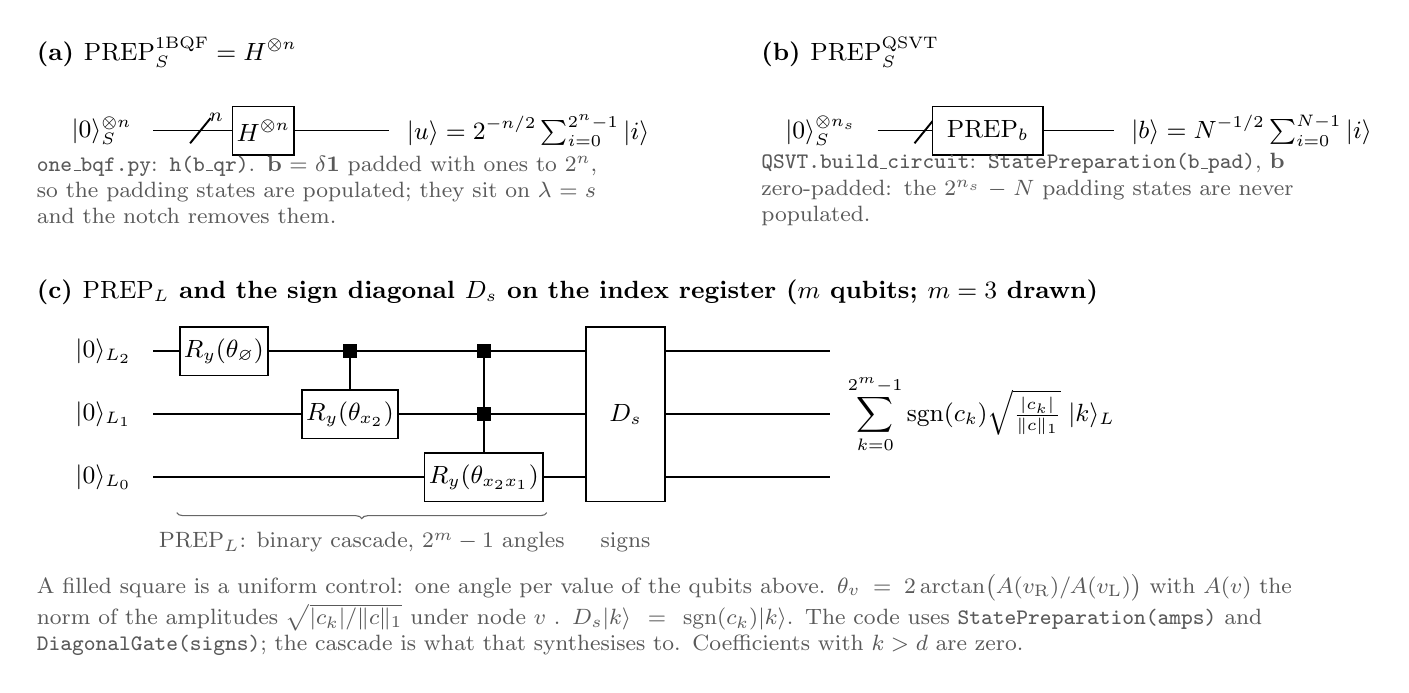
\begin{tikzpicture}[x=1cm,y=1cm]
% (a) H^n
\node[anchor=west,font=\small\bfseries] at (-1.6,1.0) {(a) $\mathrm{PREP}_S^{\rm 1BQF}=H^{\otimes n}$};
\lab{-0.15}{0}{$|0\rangle^{\otimes n}_S$}
\wires{0}{3.0}{0} \slashwire{0.6}{0}{$n$}
\gt{1.4}{0}{$H^{\otimes n}$}
\node[font=\small,anchor=west] at (3.1,0) {$|u\rangle=2^{-n/2}\sum_{i=0}^{2^n-1}|i\rangle$};
\node[font=\footnotesize,anchor=west,text=black!65,text width=7.2cm] at (-1.6,-0.75) {\texttt{one\_bqf.py}: \texttt{h(b\_qr)}. $\mathbf b=\delta\mathbf 1$ padded with ones to $2^n$, so the padding states are populated; they sit on $\lambda=s$ and the notch removes them.};
% (b) StatePreparation(b)
\begin{scope}[shift={(9.2,0)}]
\node[anchor=west,font=\small\bfseries] at (-1.6,1.0) {(b) $\mathrm{PREP}_S^{\rm QSVT}$};
\lab{-0.15}{0}{$|0\rangle^{\otimes n_s}_S$}
\wires{0}{3.0}{0} \slashwire{0.6}{0}{$n_s$}
\wg{1.4}{0}{14mm}{$\mathrm{PREP}_b$}
\node[font=\small,anchor=west] at (3.1,0) {$|b\rangle=N^{-1/2}\sum_{i=0}^{N-1}|i\rangle$};
\node[font=\footnotesize,anchor=west,text=black!65,text width=7.2cm] at (-1.6,-0.75) {\texttt{QSVT.build\_circuit}: \texttt{StatePreparation(b\_pad)}, $\mathbf b$ zero-padded: the $2^{n_s}-N$ padding states are never populated.};
\end{scope}
% (c) LCU PREP and sign diagonal, m=3 drawn
\begin{scope}[shift={(0,-3.6)}]
\node[anchor=west,font=\small\bfseries] at (-1.6,1.55) {(c) $\mathrm{PREP}_L$ and the sign diagonal $D_s$ on the index register ($m$ qubits; $m=3$ drawn)};
\lab{-0.15}{0.8}{$|0\rangle_{L_2}$} \lab{-0.15}{0}{$|0\rangle_{L_1}$} \lab{-0.15}{-0.8}{$|0\rangle_{L_0}$}
\wires{0}{8.6}{0.8,0,-0.8}
\gt{0.9}{0.8}{$R_y(\theta_\varnothing)$}
\node[rectangle,draw,fill=black,minimum size=1.6mm,inner sep=0] at (2.5,0.8) {}; \vl{2.5}{0.8}{0} \gt{2.5}{0}{$R_y(\theta_{x_2})$}
\node[rectangle,draw,fill=black,minimum size=1.6mm,inner sep=0] at (4.2,0.8) {}; \node[rectangle,draw,fill=black,minimum size=1.6mm,inner sep=0] at (4.2,0) {}; \vl{4.2}{0.8}{-0.8} \gt{4.2}{-0.8}{$R_y(\theta_{x_2x_1})$}
\mb{6.0}{0.8}{-0.8}{1.0}{$D_s$}
\node[font=\small,anchor=west] at (8.7,0) {$\displaystyle \sum_{k=0}^{2^m-1}\mathrm{sgn}(c_k)\sqrt{\tfrac{|c_k|}{\lVert c\rVert_1}}\;|k\rangle_L$};
\draw[brace] (0.3,-1.25) -- (5.0,-1.25); \node[blk] at (2.65,-1.38) {$\mathrm{PREP}_L$: binary cascade, $2^m-1$ angles};
\node[blk] at (6.0,-1.38) {signs};
\node[font=\footnotesize,anchor=west,text=black!65,text width=16.5cm] at (-1.6,-2.55) {A filled square is a uniform control: one angle per value of the qubits above. $\theta_v=2\arctan\!\big(A(v_{\rm R})/A(v_{\rm L})\big)$ with $A(v)$ the norm of the amplitudes $\sqrt{|c_k|/\lVert c\rVert_1}$ under node $v$ . $D_s|k\rangle=\mathrm{sgn}(c_k)|k\rangle$. The code uses \texttt{StatePreparation(amps)} and \texttt{DiagonalGate(signs)}; the cascade is what that synthesises to. Coefficients with $k>d$ are zero.};
\end{scope}
\end{tikzpicture}
\end{document}
